\documentclass[../sparc.tex]{subfiles}
\graphicspath{{\subfix{../images/}}}
\begin{document}

%%%%%%%%%%%%%%%%%%%%%%%%%%%%%%%%%%%%%%%%%%%%%%%%%%%%%%%%%%%%%%%%%%%%%%%%%%%%%%%%
\section{Графика}

Несмотря на то, что дисплей в нашем проекте используется текстовый, и он не даёт
нам возможности рисовать произвольные рисунки в любом месте экрана, нам доступна
возможность создавать собственные символы.  Эти символы затем можно отображать в
клетках дисплея.

Размер клетки на нашем дисплее составляет 8х5 пикселей (8 строк на 5 столбцов.)
Схематически это можно визуализировать, как показано на
рис. \ref{fig:game-dev-char}.

\begin{figure}[ht]
  \centering
  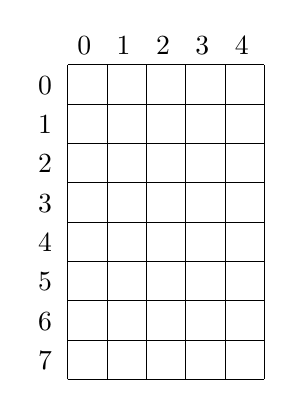
\begin{tikzpicture}
    \draw[step=0.5cm,black,very thin] (-2.5, -4) grid (0, 0);
    \foreach[count=\n from 0] \x in {-2.5, -2.0, ..., -0.5} {
      \draw (\x cm, 0) node[anchor=south west] {$\n$};
    }
    \foreach[count=\n from 0] \y in {-0.5, -1.0, ..., -4} {
      \draw (-3.0, \y) node[anchor=south west] {$\n$};
    }
  \end{tikzpicture}
  \caption{Схематическое изображение клетки, в которой отрисовывается символ.}
  \label{fig:game-dev-char}
\end{figure}

На дисплее 4 строки на 20 столбцов всего 80 таких клеток, показанных на рис.
\ref{fig:game-dev-char}.

Каждый пиксель описывается одним битом. Единица означает, что пиксель закрашен,
ноль означает, что пиксель не закрашен. Например, строчка, показанная на рис.
\ref{fig:game-dev-char-symbol-encoding}, может быть описана, как
\texttt{0b01010}.

\note{ Обратите внимание, что числа, начинающиеся с префикса \texttt{0b} (символ
  нуля и английской буквы ``b''), записаны напрямую в двоичном виде.  Не стоит
  забывать, что компьютер \emph{все} данные, которые мы сохраняем в памяти,
  хранит в двоичном виде; задавая префикс перед числом, мы лишь меняем формат
  записи числа, а не формат хранения.  Из других префиксов можно назвать
  \texttt{0x} (ноль-икс), позволяющий указывать шестнадцатиричные числа
  (например \texttt{0xFF}) и префикс \texttt{0} (ноль), позволяющий указывать
  восьмеричные числа. }

\begin{figure}[ht]
  \centering
  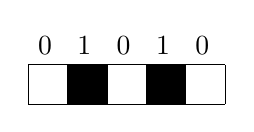
\begin{tikzpicture}
    \draw[step=0.5cm,black,very thin] (-2.5, -0.5) grid (0, 0);
    \fill[black] (-2.0, 0) rectangle (-1.5, -0.5);
    \fill[black] (-1.0, 0) rectangle (-0.5, -0.5);
    \foreach \x/\n in {-2.5/0, -2.0/1, -1.5/0, -1.0/1, -0.5/0} {
      \draw (\x cm, 0) node[anchor=south west] {$\n$};
    }
  \end{tikzpicture}
  \caption{Кодирование пикселей в одной строке символа.}
  \label{fig:game-dev-char-symbol-encoding}
\end{figure}

Одна строка символа кодируется одним байтом информации (восемью битами) из
которых фактически используется только пять младших бит.

\end{document}
